%!TEX program = xelatex
% 完整编译: xelatex -> bibtex -> xelatex -> xelatex
\documentclass[lang=cn,10pt,a4paper,cite=authoryear]{elegantpaper}

\title{统计学习实验三:Logistics Regression}
\author{王嗣萱 2018110601014}
\date{}


% 本文档命令
\usepackage{array}
\newcommand{\ccr}[1]{\makecell{{\color{#1}\rule{1cm}{1cm}}}}

\begin{document}

\maketitle

\section{实验原理}

\subsection{Logistic 分布}
Logistic 分布是一种连续型的概率分布,其分布函数和密度函数分别为:

$F(x) = P(X \leq x)=\frac{1}{1+e^{-(x-\mu)/\gamma}} $

$ f(x) = F^{'}(X \leq x)=\frac{e^{-(x-\mu)/\gamma}}{\gamma(1+e^{-(x-\mu)/\gamma})^{2}}$

其中, $\mu$ 表示位置参数, $\gamma$ 为形状参数。我们可以看下其图像特征:

\begin{figure}[htbp]
	\centering
	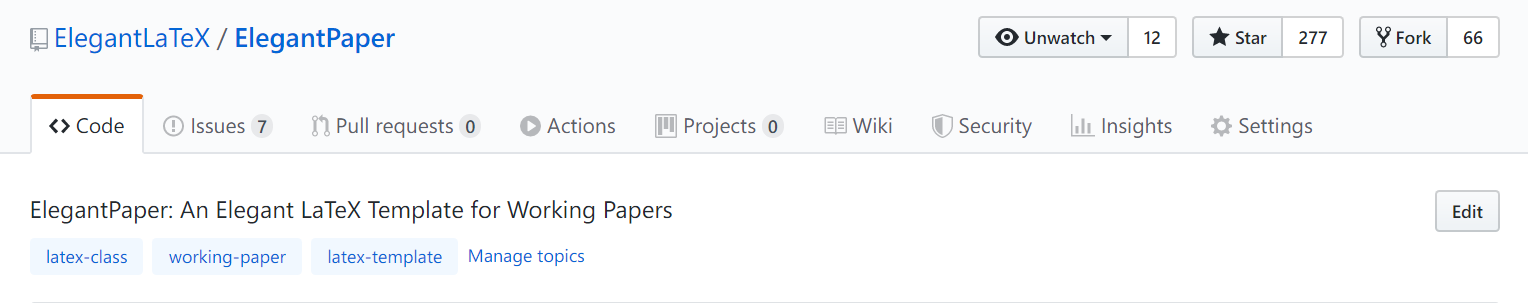
\includegraphics[width=\textwidth]{star.png}
	\caption{一键三连求赞}
\end{figure}
\subsection{Logistic 回归}

\subsection{}

\section{Python代码实现}

\section{结果及图形展示}

\section{总结体会}

\end{document}
